\chapter{Θεωρητικό υπόβαθρο}\label{ch:theory}

\section{Εισαγωγή στην Μηχανική Μάθηση}\label{sec:ml}
\subsection{Μηχανική Μάθηση}\label{ssec:ml-def}
Η Μηχανική Μάθηση (Machine Learning, ML) είναι ένα ερευνητικό πεδίο της Τεχνητής Νοημοσύνης που εστιάζει στην ανάπτυξη αλγορίθμων και μοντέλων που έχουν την ικανότητα να εξάγουν γνώση από σύνολα δεδομένων και να την εφαρμόζουν σε νέες, άγνωστες εισόδους, χωρίς να απαιτούν ρητό προγραμματισμό για κάθε ενέργεια \cite{mitchell_machine_1997, flach_machine_2012}. Για να επιτευχθεί αυτό, αξιοποιούνται διάφορες στατιστικές μέθοδοι αναγνώρισης και εξαγωγής προτύπων. Η θεμελιώδης διαφορά της Μηχανικής Μάθησης από τον κλασικό προγραμματισμό έγκειται στην αρχιτεκτονική της: αντί να χρησιμοποιηθούν αυστηροί ντετερμινιστικοί κανόνες if-then και αναλυτικοί υπολογισμοί, αναπτύσσονται στοχαστικά μοντέλα τα οποία αφομοιώνουν πληροφορία από μεγάλο όγκο δεδομένων μέσω μιας διαδικασίας που ονομάζεται «εκπαίδευση» (training) και εκφράζουν τα αποτελέσματα της ανάλυσής τους πιθανοκρατικά.

Κάποια από τα προβλήματα που επιλύουν μοντέλα Μηχανικής Μάθησης είναι η ταξινόμηση (classification), ο διαχωρισμός δηλαδή των δεδομένων σε δύο ή περισσότερες κλάσεις βάσει των χαρακτηριστικών τους, η στατιστική παλινδρόμηση (regression), όπου μελετάται η συσχέτιση μίας εξαρτημένης τυχαίας μεταβλητής με μία ή περισσότερες ανεξάρτητες, με σκοπό την πρόβλεψη μελλοντικών σχέσεων μεταξύ τους, και η μείωση διαστατικότητας (dimensionality reduction), η οποία στοχεύει στην έκφραση δεδομένων από έναν χώρο πολλών διαστάσεων σε έναν μικρότερο, διατηρώντας όσο το δυνατόν περισσότερα από τα αρχικά τους χαρακτηριστικά \cite{bishop_pattern_2006, michie_machine_1995}.

Οι μέθοδοι Μηχανικής Μάθησης διακρίνονται σε τρεις γενικές κατηγορίες: την επιτηρούμενη ή επιβλεπόμενη μάθηση (supervised learning), όπου τα επιθυμητά αποτελέσματα εξόδου (ετικέτες) δίνονται εκ των προτέρων στο πρόγραμμα με στόχο να αντιστοιχηθούν μέσω κάποιου κανόνα με τα δεδομένα εισόδου, την μη επιτηρούμενη ή μη επιβλεπόμενη μάθηση (unsupervised learning), στην οποία το πρόγραμμα καλείται να ανακαλύψει κρυφά μοτίβα από τα δεδομένα χωρίς να του δοθούν ενδεικτικά αποτελέσματα, και την ενισχυτική μάθηση (reinforcement learning), στην οποία το πρόγραμμα εξερευνά δυναμικά τον χώρο του προβλήματος και δέχεται σήματα επιβράβευσης ή ποινής ανάλογα με το πόσο κοντά βρίσκεται στον στόχο του \cite{mitchell_machine_1997, bishop_pattern_2006}.

\begin{figure}[htbp]
  \centering
  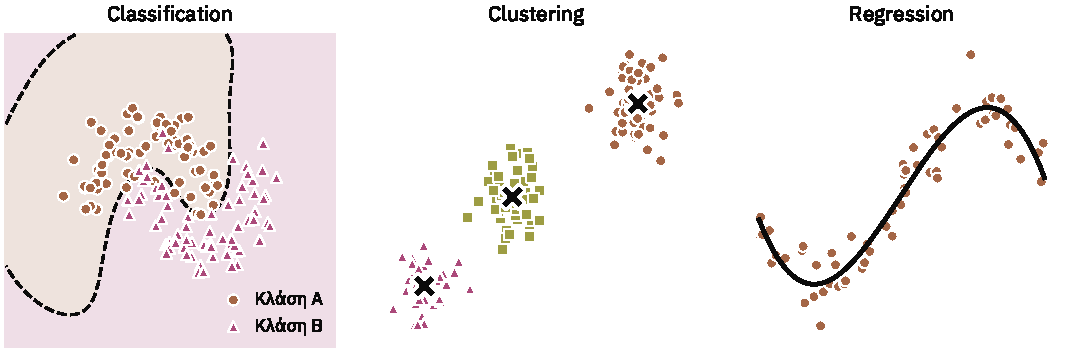
\includegraphics[width=\linewidth]{./assets/images/ml-overview}
  \caption[Θεμελιώδη προβλήματα μηχανικής μάθησης]{Τρία προβλήματα μηχανικής μάθησης: η ταξινόμηση (classification) και η παλινδρόμηση (regression), που αποτελούν επιβλεπόμενα tasks, και η ομαδοποίηση (clustering), ένα μη επιβλεπόμενο task.}
  \label{fig:ml-overview}
\end{figure}

\subsection{Νευρωνικά Δίκτυα}\label{ssec:nn}
Μία από τις παλαιότερες αλλά και πλέον διαδεδομένες αρχιτεκτονικές της Μηχανικής Μάθησης είναι τα Τεχνητά Νευρωνικά Δίκτυα, ή απλώς Νευρωνικά Δίκτυα (Neural Networks, NNs). Εισήχθησαν το 1943 από τους McCulloch και Pitts, σε μια προσπάθεια να προσομοιώσουν μαθηματικά τους βιολογικούς νευρώνες του εγκεφάλου \cite{mcculloch_logical_1943}, ενώ αναπτύχθηκαν περαιτέρω το 1958 από τον Rosenblatt με την εισαγωγή του perceptron \cite{rosenblatt_perceptron_1958}.

Ένα Νευρωνικό Δίκτυο απαρτίζεται από υπολογιστικούς κόμβους (νευρώνες), συνδεδεμένους μεταξύ τους και οργανωμένους σε επίπεδα (layers). Η βασική αρχιτεκτονική περιλαμβάνει ένα επίπεδο εισόδου, ένα επίπεδο εξόδου, και ένα ή περισσότερα ενδιάμεσα (κρυφά) επίπεδα ανάμεσά τους, όπου συντελείται η επεξεργασία της πληροφορίας (\autoref{fig:mlp}). Η είσοδος κάθε νευρώνα προκύπτει από τις εξόδους των νευρώνων του προηγούμενου επιπέδου με τους οποίους συνδέεται. Οι τιμές αυτές πολλαπλασιάζονται με κατάλληλους συντελεστές βάρους (weights), αθροίζονται, και το αποτέλεσμα διέρχεται από μία μη γραμμική συνάρτηση ενεργοποίησης, η οποία καθορίζει το τελικό σήμα εξόδου του νευρώνα \cite{goodfellow_deep_2016}.

\begin{figure}[ht]
  \centering
  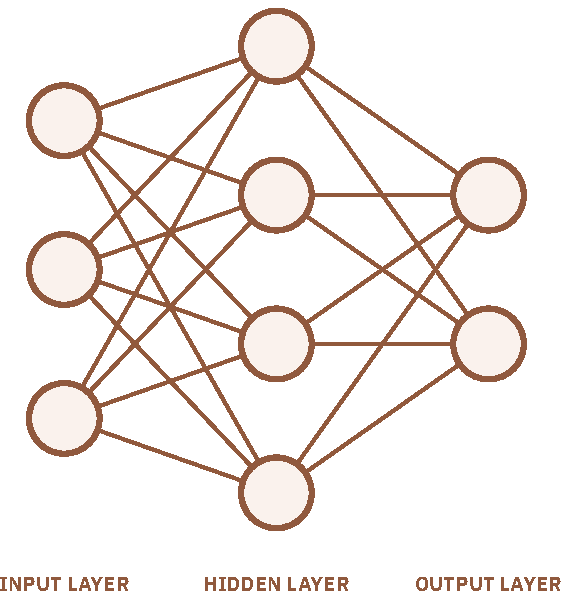
\includegraphics[width=0.5\linewidth]{./assets/images/mlp}
  \caption[Βασική δομή MLP]{Η βασική δομή ενός πλήρως συνδεδεμένου νευρωνικού δικτύου (MLP): επίπεδο εισόδου, κρυφά επίπεδα και επίπεδο εξόδου. Στο συγκεκριμένο παράδειγμα φαίνεται ένα κρυφό επίπεδο.}
  \label{fig:mlp}
\end{figure}

Οι εφαρμογές των Νευρωνικών Δικτύων είναι ποικίλες, εκτεινόμενες από την επεξεργασία εικόνας και την πρόβλεψη χρονοσειρών, μέχρι τα συστήματα σύστασης (recommender systems) \cite{lecun_deep_2015}, με τα οποία καταπιάνεται η παρούσα διπλωματική εργασία.

\subsection{Η διαδικασία εκπαίδευσης}\label{ssec:training}
Η εκπαίδευση των Νευρωνικών Δικτύων στηρίζεται σε μία επαναληπτική διαδικασία μαθηματικής βελτιστοποίησης. Προκειμένου το μοντέλο να αξιολογήσει την απόδοσή του, ορίζεται μία συνάρτηση σφάλματος (loss function), η οποία ποσοτικοποιεί την απόκλιση μεταξύ της τρέχουσας πρόβλεψης του δικτύου και του πραγματικού επιθυμητού αποτελέσματος. Στην αρχή της εκπαίδευσης, οι παράμετροι (βάρη) του μοντέλου αρχικοποιούνται με τυχαίες τιμές, οδηγώντας σε σχεδόν τυχαίες προβλέψεις και, επομένως, σε υψηλό σφάλμα. Σε κάθε επόμενο γύρο εκπαίδευσης, το μοντέλο υπολογίζει την κλίση (gradient) της συνάρτησης σφάλματος ως προς κάθε βάρος. Οι κλίσεις αυτές υποδεικνύουν την κατεύθυνση προς την οποία πρέπει να αναπροσαρμοστούν τα βάρη ώστε το σφάλμα να ελαχιστοποιηθεί. Το πόσο μεγάλη θα είναι η αναπροσαρμογή αυτή καθορίζεται από μία υπερπαράμετρο της εκπαίδευσης, τον ρυθμό μάθησης (learning rate). Η επαναληπτική αυτή διαδικασία είναι ευρέως γνωστή ως Gradient Descent \cite{mitchell_machine_1997}. Με σωστή επιλογή παραμέτρων εκπαίδευσης και ικανό αριθμό επαναλήψεων, η διαδικασία συγκλίνει, με αποτέλεσμα το μοντέλο να μάθει τα λανθάνοντα μοτίβα των δεδομένων.

Η πιο συνήθης μέθοδος οργάνωσης και ενορχήστρωσης αυτής της διαδικασίας είναι η κεντρικοποιημένη (centralized learning), στην οποία όλα τα δεδομένα προς εκπαίδευση συγκεντρώνονται σε έναν κεντρικό διακομιστή (server), από όπου και τροφοδοτούνται στο μοντέλο. Αυτή η μέθοδος είναι αρχιτεκτονικά απλή και, συνήθως, υπολογιστικά αποδοτική, αφενός επειδή το μοντέλο εκπαιδεύεται στο πλήρες, πληροφοριακά πυκνό σύνολο δεδομένων, και αφετέρου γιατί δεν χρειάζονται επιπλέον επίπεδα επικοινωνίας για την ανανέωση και την μετάδοση των βαρών του. Ωστόσο, αυτή η απλότητα έρχεται με ένα κόστος. Η συγκέντρωση μεγάλου όγκου δεδομένων σε έναν κόμβο δημιουργεί ένα εξαιρετικά ευάλωτο σημείο αποτυχίας. Μία πιθανή κακόβουλη επίθεση στον κεντρικό διακομιστή αρκεί για να παραβιαστούν τα προσωπικά δεδομένα χιλιάδων χρηστών \cite{kairouz_advances_2021}, γεγονός που καθιστά την κεντρικοποιημένη αρχιτεκτονική ακατάλληλη για εφαρμογές που πραγματεύονται ευαίσθητα προσωπικά δεδομένα, όπως ιατρικό ιστορικό ή τραπεζικούς λογαριασμούς.

\section{Εισαγωγή στην Ομοσπονδιακή Μάθηση}\label{sec:fl}
\subsection{Εισαγωγή στο IoT}\label{ssec:iot}
Το Διαδίκτυο των Πραγμάτων (Internet of Things, IoT) είναι ένας από τους ταχύτερα αναπτυσσόμενους τομείς εμπορικά διαθέσιμων τεχνολογιών στις μέρες μας. Αφορά την ανάπτυξη «έξυπνων» συσκευών οικιακής χρήσης όπως λαμπτήρες, κάμερες ασφαλείας, θερμοστάτες, πρίζες κτλ, οι οποίες επικοινωνούν μεταξύ τους μέσω του διαδικτύου, καθιστώντας έτσι δυνατή την αυτοματοποίησή τους \cite{atzori_internet_2010}. Για παράδειγμα, μία έξυπνη κάμερα ασφαλείας μπορεί να ειδοποιήσει τον χρήστη στο κινητό του όταν εντοπίσει κάποιο πρόσωπο στην είσοδο, ή μία προγραμματισμένη έξυπνη πρίζα μπορεί να ενεργοποιήσει τη θέρμανση λίγο πριν γυρίσει ο χρήστης στο σπίτι.

Όπως γίνεται αντιληπτό, η λειτουργία τέτοιων αυτοματισμών αντλεί ευαίσθητα προσωπικά δεδομένα χρηστών, όπως το ωράριο εργασίας τους, την τοποθεσία τους ή τα βιομετρικά τους χαρακτηριστικά. Επιπλέον, συνήθως απαιτείται ταυτοποίηση του χρήστη μέσω email ή αριθμού τηλεφώνου, καθώς και παραχώρηση πρόσβασης στο τοπικό του δίκτυο, πληροφορίες εξίσου ευαίσθητες. Η προσπάθεια κεντρικοποιημένης επεξεργασίας αυτών των δεδομένων για την εκπαίδευση μοντέλων Μηχανικής Μάθησης εγείρει προφανείς κινδύνους ασφαλείας. Για τον λόγο αυτό εισάγεται ένας νέος τρόπος εκπαίδευσης μοντέλων Μηχανικής Μάθησης, η Ομοσπονδιακή Μάθηση.

\subsection{Ομοσπονδιακή Μάθηση}\label{ssec:fl}
Η βασική αρχή της Ομοσπονδιακής Μάθησης (Federated Learning, FL), έγκειται στο γεγονός ότι τα προσωπικά δεδομένα κάθε χρήστη παραμένουν αποκλειστικά στην διάθεσή του. Για να επιτευχθεί αυτός ο στόχος, αντί να μεταφερθούν τα δεδομένα των χρηστών σε έναν κεντρικό υπολογιστή για την εκπαίδευση του μοντέλου, μεταφέρεται το μοντέλο στην συσκευή κάθε χρήστη, όπου εκπαιδεύεται τοπικά, χωρίς να διαμοιραστεί τα δεδομένα του \cite{mcmahan_communication-efficient_2017}. Ο κεντρικός server λαμβάνει και αποθηκεύει αποκλειστικά τις παραμέτρους (βάρη) του δικτύου, οι οποίες αποτελούν ανώνυμες αριθμητικές μεταβλητές που δεν περιέχουν καμία πληροφορία για τους χρήστες.

Η αρχιτεκτονική της εκπαίδευσης χωρίζεται σε δύο είδη οντοτήτων: τον κεντρικό διακομιστή (server), υπεύθυνο για την ενορχήστρωση της διαδικασίας και την αποθήκευση ενός κεντρικού, καθολικού μοντέλου (global model), και τους χρήστες/πελάτες (clients), οι οποίοι διαθέτουν τα τοπικά τους προσωπικά δεδομένα, και εκπαιδεύουν τα δικά τους τοπικά μοντέλα (local models), τα βάρη των οποίων συναθροίζονται για να απαρτίσουν το κεντρικό μοντέλο (\autoref{fig:centralized-vs-federated}) \cite{yang_federated_2019}.

\begin{figure}[htbp]
  \centering
  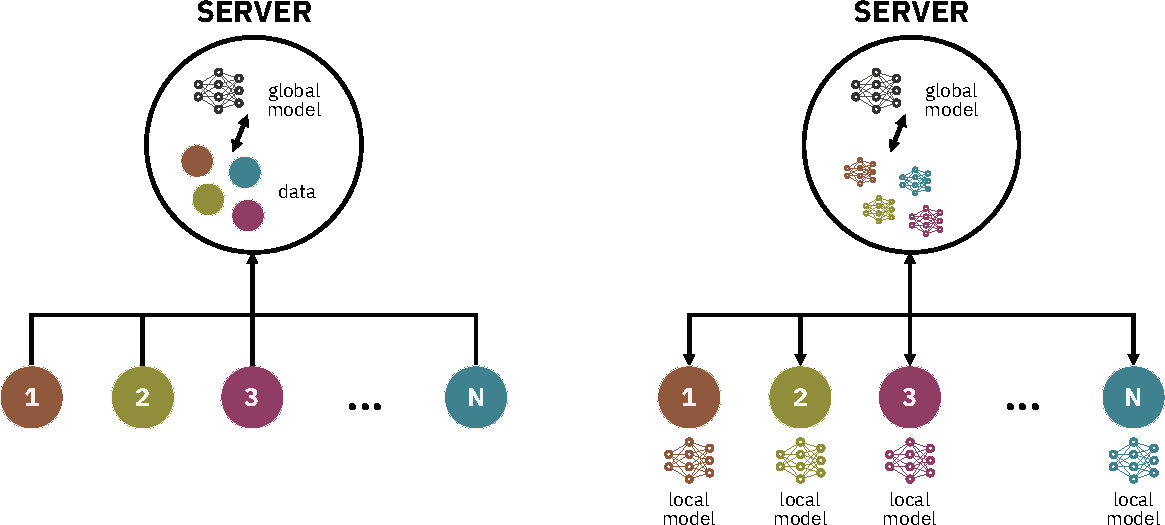
\includegraphics[width=\linewidth]{./assets/images/centralized-vs-federated}
  \caption[Centralized vs. Federated Learning]{Σύγκριση κεντρικοποιημένης (αριστερά) και ομοσπονδιακής (δεξιά) μάθησης: στην πρώτη τα δεδομένα συγκεντρώνονται στον server, ο οποίος εκπαιδεύει ένα κεντρικό μοντέλο, ενώ στη δεύτερη οι clients αποστέλλουν μόνο τα βάρη των τοπικών τους μοντέλων και ποτέ τα ίδια τους τα δεδομένα.}
  \label{fig:centralized-vs-federated}
\end{figure}

Η διαδικασία της εκπαίδευσης παρουσιάζει κάποιες διαφορές σε σχέση με την κλασική centralized υλοποίηση, μιας και πλέον αξιοποιείται η συσκευή κάθε χρήστη. Η εκπαίδευση εκτυλίσσεται σε γύρους επικοινωνίας (communication rounds) \cite{bonawitz_towards_2019}. Αρχικά, ο server μεταδίδει το τρέχον καθολικό μοντέλο σε μέρος (ή στην πληρότητα) των clients προς εκπαίδευση. Ο κάθε client εκπαιδεύει το μοντέλο τοπικά, όχι στο σύνολο των δεδομένων όλων των χρηστών (καθώς δεν έχει πρόσβαση σε αυτά), αλλά αποκλειστικά στα δικά του, τοπικά δεδομένα. Όπως και στην centralized εκπαίδευση, ο κάθε client πραγματοποιεί gradient descent (βλ. \autoref{ssec:training}). Ανάλογα με την φύση του προβλήματος προς επίλυση, μπορεί ο κάθε client να εκτελέσει έναν ή περισσότερους τέτοιους γύρους τοπικής εκπαίδευσης. Αφού κάθε client έχει ολοκληρώσει αυτό το στάδιο, αποστέλλει τα ανανεωμένα βάρη του μοντέλου (ή τις διαφορές τους) πίσω στον server. Ο server, με τη σειρά του, χρησιμοποιεί μια συνάρτηση συνάθροισης (aggregation function) για να συγχωνεύσει τις τοπικές ενημερώσεις σε ένα νέο, βελτιωμένο καθολικό μοντέλο. Η συνάρτηση αυτή μπορεί να έχει οποιαδήποτε μορφή κατά περίπτωση, αλλά συνήθως χρησιμοποιείται ο σταθμισμένος μέσος όρος (Federated Averaging, FedAvg) \cite{mcmahan_communication-efficient_2017}. Σε αυτό το σημείο ολοκληρώνεται ένας γύρος επικοινωνίας και ξεκινάει ο επόμενος. Ο server στέλνει τα νέα, μεσοσταθμισμένα βάρη του μοντέλου στους clients, εκείνοι πραγματοποιούν κάποιους γύρους τοπικής εκπαίδευσης, αποστέλλουν πίσω τα νέα τους βάρη και ο server τα συναθροίζει. Μετά από κάποιον αριθμό επαναλήψεων, το μοντέλο συγκλίνει σε μία λύση που εκφράζει όλους τους clients σε κάποιο βαθμό, χωρίς να έχει εκπαιδευτεί ποτέ στο σύνολο των δεδομένων τους αυτούσιο. Τα στάδια της διαδικασίας απεικονίζονται στο \autoref{fig:fl-pipeline}.

\begin{figure}[htbp]
  \centering
    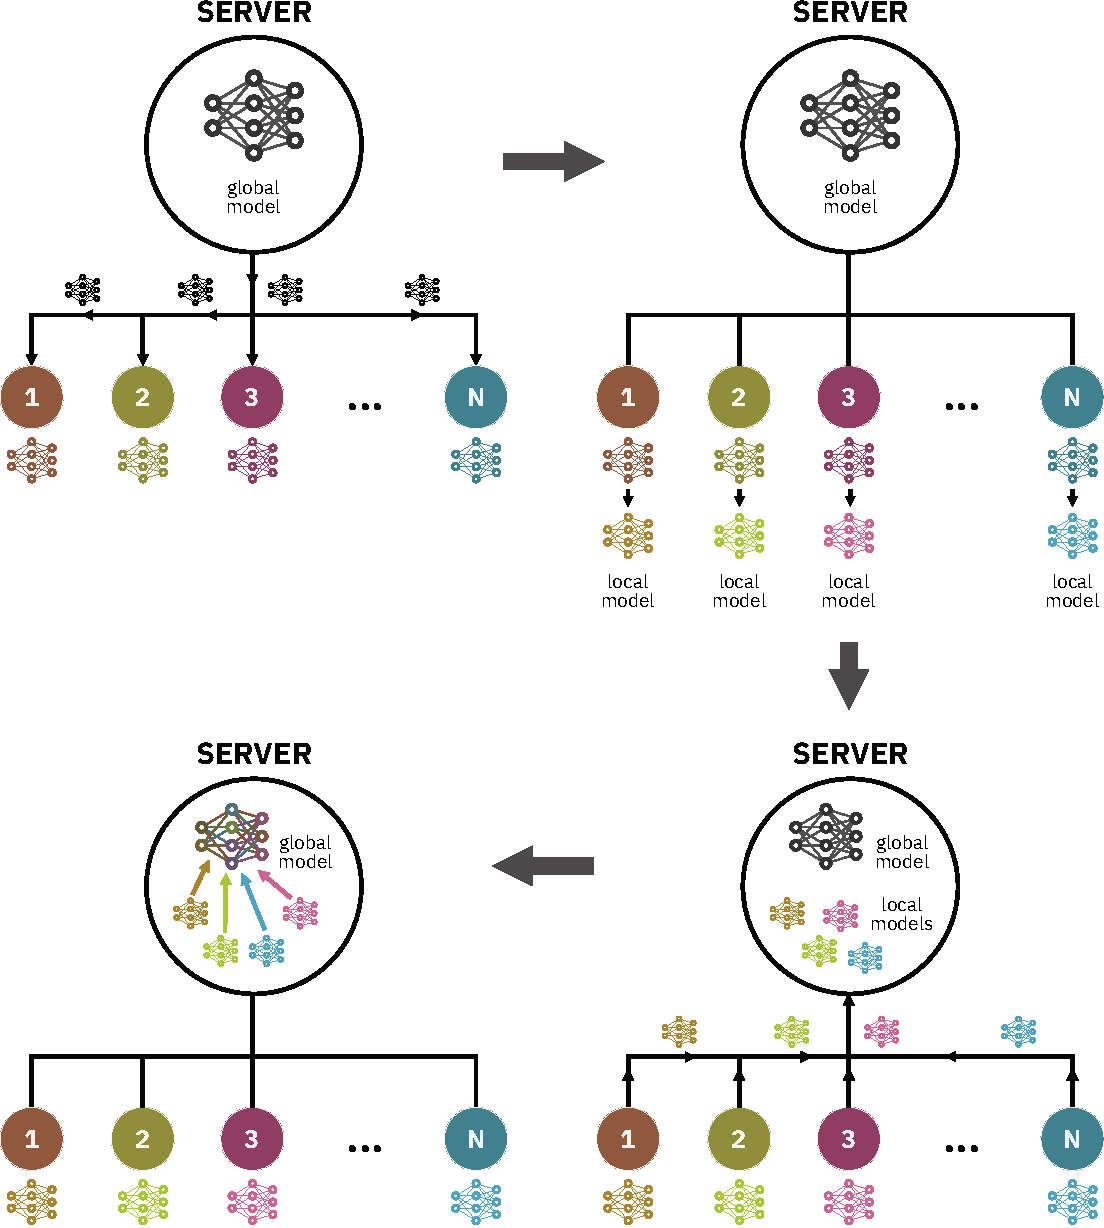
\includegraphics[width=\linewidth]{./assets/images/fl-pipeline}
  \caption[Pipeline ομοσπονδιακής μάθησης]{Το pipeline ενός γύρου επικοινωνίας: \textbf{(α) πάνω αριστερά:} ο server μεταδίδει το global μοντέλο στους clients, \textbf{(β) πάνω δεξιά:} οι clients εκπαιδεύουν τοπικά τα μοντέλα τους, \textbf{(γ) κάτω δεξιά:} τα ανανεωμένα βάρη αποστέλλονται πίσω στον server, \textbf{(δ) κάτω αριστερά:} ο server κάνει aggregate τα βάρη στο global μοντέλο.}
  \label{fig:fl-pipeline}
\end{figure}

Αυτή η ιδιότητα ωστόσο της federated αρχιτεκτονικής συχνά εισάγει ένα σημαντικό πρόβλημα: τα δεδομένα των χρηστών τείνουν να είναι στατιστικά ετερογενή \cite{li_federated_2020}. Σε αντίθεση με τις κεντρικοποιημένες βάσεις δεδομένων, τα δεδομένα των αυτόνομων clients δεν είναι Ανεξάρτητα και Ταυτόσημα Κατανεμημένα (Independent and Identically Distributed, IID), δηλαδή δεν είναι ισορροπημένα ούτε ως προς τον όγκο ούτε ως προς την φύση της πληροφορίας που περιέχουν. Για παράδειγμα, το ιατρικό ιστορικό σε μία ορθοπεδική κλινική αποτελείται κυρίως από ορθοπεδικά περιστατικά, ενώ σε ένα γενικό νοσοκομείο υπάρχει σαφώς μεγαλύτερη γκάμα παθήσεων, και σαφώς περισσότερα περιστατικά συνολικά. Λόγω αυτής της στατιστικής ανισορροπίας, τα τοπικά μοντέλα τείνουν να συγκλίνουν προς εντελώς διαφορετικές, τοπικά βέλτιστες κατευθύνσεις. Όταν ο server επιχειρεί να αθροίσει αυτές τις αποκλίνουσες παραμέτρους, το καθολικό μοντέλο παρουσιάζει αστάθεια και συχνά αδυνατεί να συγκλίνει. Το φαινόμενο αυτό αναφέρεται στην βιβλιογραφία ως client drift (\autoref{fig:client-drift}) \cite{karimireddy_scaffold_2020, li_federated_2020} και αντιμετωπίζεται με διάφορες αλγοριθμικές τεχνικές, οι οποίες θα αναλυθούν εκτενέστερα στην \autoref{sec:data}.

\begin{figure}[htbp]
  \centering
  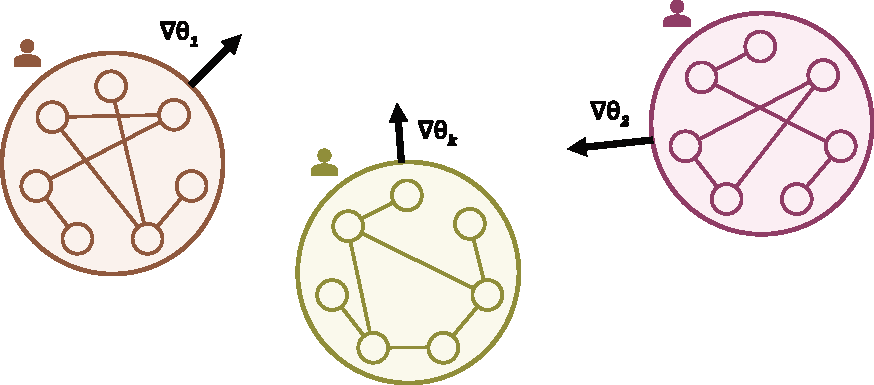
\includegraphics[width=\linewidth]{./assets/images/client-drift}
  \caption[Client drift]{Client drift: κάθε τοπικό μοντέλο παράγει gradient σε διαφορετική κατεύθυνση, με αποτέλεσμα το καθολικό μοντέλο να είναι ασταθές.}
  \label{fig:client-drift}
\end{figure}

Κλείνοντας την εισαγωγή στην Ομοσπονδιακή Μάθηση, αξίζει να σημειωθεί μία ακόμη αρχιτεκτονική λεπτομέρεια: η διαφοροποίηση μεταξύ Cross-Device FL και Cross-Silo FL (\autoref{fig:cross-device-vs-cross-silo}) \cite{kairouz_advances_2021}. Μέχρι τώρα έγινε αναφορά στην εκπαίδευση ενός ξεχωριστού τοπικού μοντέλου στην συσκευή κάθε χρήστη/client (cross-device FL). Σε μερικές εφαρμογές ωστόσο επιστρατεύεται η αρχιτεκτονική cross-silo FL, η οποία λειτουργεί ως ένας συμβιβασμός μεταξύ της πλήρως centralized και της πλήρως federated υλοποίησης. Σε αυτή τη δομή, τα δεδομένα ομαδοποιούνται (ή βρίσκονται ήδη) τοπικά σε αξιόπιστους «υπερκόμβους» (supernodes) ή «σιλό» οργανισμών (π.χ. νοσοκομεία ή περιφερειακοί διακομιστές) και επεξεργάζονται μαζικά (ως batch). Η αρχιτεκτονική cross-device απαιτεί τον συντονισμό χιλιάδων ή εκατομμυρίων συσκευών, μερικές εκ των οποίων μπορεί να είναι ασταθείς, ωστόσο προσφέρει την μέγιστη διασφάλιση ιδιωτικότητας, ενώ η cross-silo αρχιτεκτονική προσφέρει ευκολότερη και σταθερότερη ενορχήστρωση, με κόστος την συγκέντρωση των δεδομένων χρηστών σε κόμβους, μακριά από την συσκευή κάθε χρήστη. Συνήθως ο τύπος ενορχήστρωσης καθορίζεται από την φύση της εφαρμογής, το πλήθος των δεδομένων και την διαθεσιμότητα του δικτύου.

\begin{figure}[htbp]
  \centering
  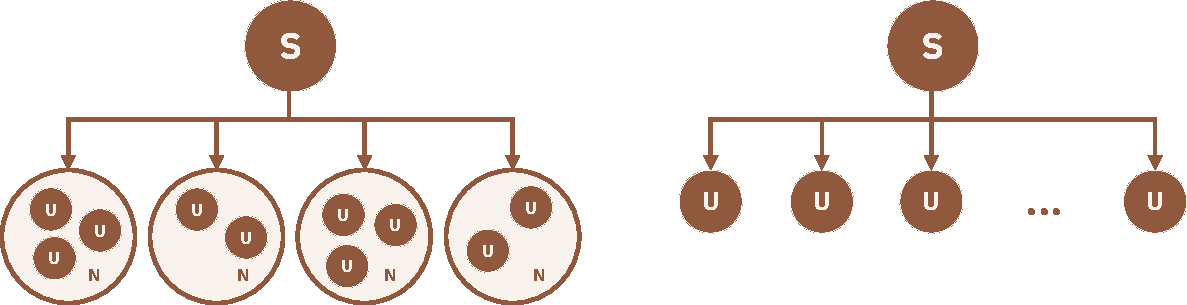
\includegraphics[width=\linewidth]{./assets/images/cross-device-vs-cross-silo}
  \caption[Cross-silo FL vs. cross-device FL]{Cross-silo FL (αριστερά): ο server \textbf{S} συνδέεται με τους υπερκόμβους \textbf{N}, καθένας από τους οποίους εξυπηρετεί τους τελικούς χρήστες \textbf{U}. Cross-device FL (δεξιά): ο server \textbf{S} συνδέεται απευθείας με τους τελικούς χρήστες \textbf{U}.}
  \label{fig:cross-device-vs-cross-silo}
\end{figure}

\section{Εισαγωγή στην Θεωρία Γράφων}\label{sec:graphs}
Σε αυτή την Ενότητα θα παρουσιαστούν συνοπτικά τα βασικά στοιχεία των Γράφων, μιας μαθηματικής αναπαράστασης εξαιρετικά χρήσιμης για την επίλυση πολλών προβλημάτων, και βασικό συστατικό στην παρούσα εργασία.

Οι Γράφοι (Graphs) αποτελούν μια δομή δεδομένων που χρησιμοποιείται στα μαθηματικά και στην επιστήμη υπολογιστών για να αναπαραστήσει πολύπλοκες σχέσεις μεταξύ οντοτήτων. Συγκεκριμένα, τα βασικά στοιχεία ενός γράφου είναι οι κόμβοι (nodes/vertices), που αναπαριστούν τα σημεία/οντότητες, και οι ακμές (edges), που αναπαριστούν τις συνδέσεις μεταξύ των κόμβων. Ένας αυστηρός μαθηματικός ορισμός \cite{wilson_introduction_1996} είναι ο εξής:

Ένας απλός γράφος $G=(\mathcal{V},\mathcal{E})$ αποτελείται από ένα μη κενό, πεπερασμένο σύνολο $\mathcal{V}$ στοιχείων που ονομάζονται κόμβοι, καθώς και από ένα πεπερασμένο σύνολο $\mathcal{E}$ που αποτελείται από διακριτά, μη διατεταγμένα ζεύγη $\{v_i, v_j\}$ στοιχείων του $\mathcal{V}$, τα οποία ονομάζονται ακμές.

Ένας γράφος μπορεί να ταξινομηθεί ως κατευθυνόμενος (directed), όταν οι ακμές μεταξύ των κόμβων του έχουν ορισμένο προσανατολισμό (από έναν κόμβο-πηγή σε έναν κόμβο-στόχο), ή μη κατευθυνόμενος (undirected) εάν οι συνδέσεις είναι συμμετρικές. Οι γράφοι μπορούν να ταξινομηθούν περαιτέρω βάσει της τοπολογίας τους (π.χ. πλήρεις γράφοι, δένδρα, κυκλικοί γράφοι κ.ά.) \cite{wilson_introduction_1996}, ωστόσο η παρούσα εργασία επικεντρώνεται στην ανάλυση απλών κατευθυνόμενων γράφων.

\begin{figure}[htbp]
  \centering
  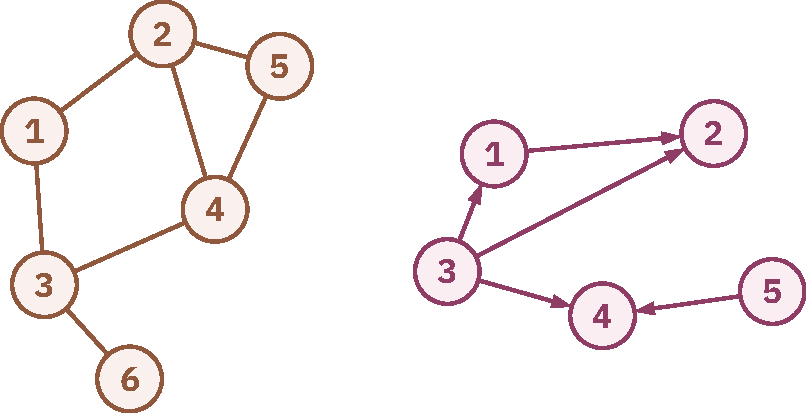
\includegraphics[width=0.8\linewidth]{./assets/images/graph-example}
  \caption[Παραδείγματα γράφων]{Παραδείγματα γράφων: μη κατευθυνόμενος γράφος με 6 κόμβους και 7 ακμές (αριστερά) και κατευθυνόμενος γράφος με 5 κόμβους και 5 ακμές (δεξιά).}
  \label{fig:graph-example}
\end{figure}

Η απλότητα αυτής της δομής παρέχει μια ευελιξία στην γκάμα των εφαρμογών που μπορεί να μοντελοποιήσει. Αυτό επιτυγχάνεται μέσω της αντιστοίχισης ενός διανύσματος χαρακτηριστικών (feature vector) στους κόμβους ή/και στις ακμές ενός γράφου, που περιγράφει εσωτερικές ιδιότητες, λειτουργίες, μοτίβα και κανόνες που επικρατούν μεταξύ τους. Για παράδειγμα, εάν αντιστοιχίσουμε τους κόμβους ενός γράφου σε ερευνητές και τις ακμές σε κοινές ακαδημαϊκές δημοσιεύσεις, προκύπτει ένας γράφος συνεργασιών που αναδεικνύει λανθάνοντα μοτίβα της ακαδημαϊκής κοινότητας.

Ο μηχανισμός αυτός αξιοποιείται στο πλαίσιο της παρούσας εργασίας για να περιγράψει τα συστήματα IoT. Εάν μοντελοποιήσουμε το σύνολο των IoT συσκευών ενός χρήστη ως έναν γράφο (\autoref{fig:typed-graph}), όπου κάθε κόμβος αποτελεί μία διακριτή συσκευή (π.χ. κάμερα ασφαλείας, έξυπνος λαμπτήρας) και κάθε ακμή έναν κανόνα αυτοματοποίησης μεταξύ τους (π.χ. αν εντοπιστεί κίνηση → άναψε), τότε μπορούμε να περιγράψουμε με μεγάλη σαφήνεια τις σχέσεις αλληλεπίδρασης των συσκευών ενός χρήστη και να εξάγουμε αποτελέσματα για τον τρόπο λειτουργίας κάθε συσκευής, μελετώντας αποκλειστικά την μορφή του γράφου.

\begin{figure}[htbp]
  \centering
  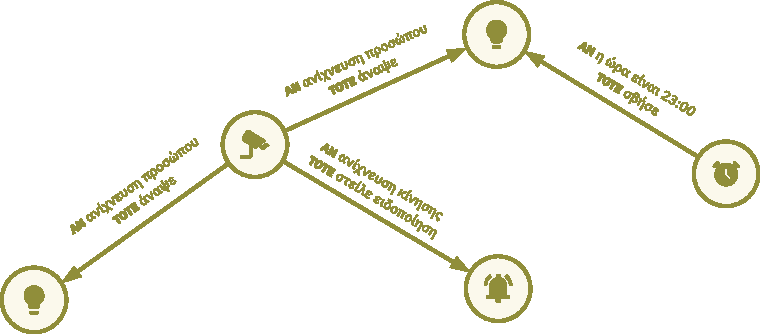
\includegraphics[width=\linewidth]{./assets/images/typed-graph}
  \caption[Γράφος με τύπους ακμών και κόμβων]{Γράφος IoT συσκευών με τύπους ακμών και κόμβων: κάθε κόμβος περιέχει το μοντέλο της συσκευής και κάθε ακμή έναν κανόνα.}
  \label{fig:typed-graph}
\end{figure}

\section{Graph Neural Networks (GNNs)}\label{sec:gnn}
Τα κλασικά Νευρωνικά Δίκτυα που παρουσιάστηκαν στην \autoref{ssec:nn} έχουν την δυνατότητα να επεξεργάζονται δεδομένα σε μορφή διανυσμάτων, πινάκων, και, κατ’ επέκταση εικόνων, ωστόσο δεν είναι εγγενώς συμβατά με την δομή των γράφων που περιγράφηκε παραπάνω, καθώς δεν μπορούν να αναπαραστήσουν την τοπολογική σύνδεση μεταξύ γειτονικών κόμβων. Για τον λόγο αυτό εισήχθη μία παραλλαγή των κλασικών Νευρωνικών Δικτύων, τα Graph Neural Networks (GNNs) \cite{scarselli_graph_2009}. Τα GNNs εντάσσονται στον ευρύτερο ερευνητικό τομέα του graph representation learning, ο οποίος περιλαμβάνει αλγορίθμους αναπαράστασης της δομής των γράφων με μορφή διανυσμάτων, όπως ο node2vec \cite{grover_node2vec_2016} και ο DeepWalk \cite{perozzi_deepwalk_2014}. Σκοπός αυτών των τεχνικών είναι να κωδικοποιήσουν την πληροφορία των features των κόμβων, καθώς και την τοπολογία του γράφου, σε διανύσματα σταθερού μεγέθους, αντιληπτά από αλγορίθμους βαθιάς μάθησης. Αυτή η διαδικασία ονομάζεται graph embedding.

\begin{figure}[htbp]
  \centering
  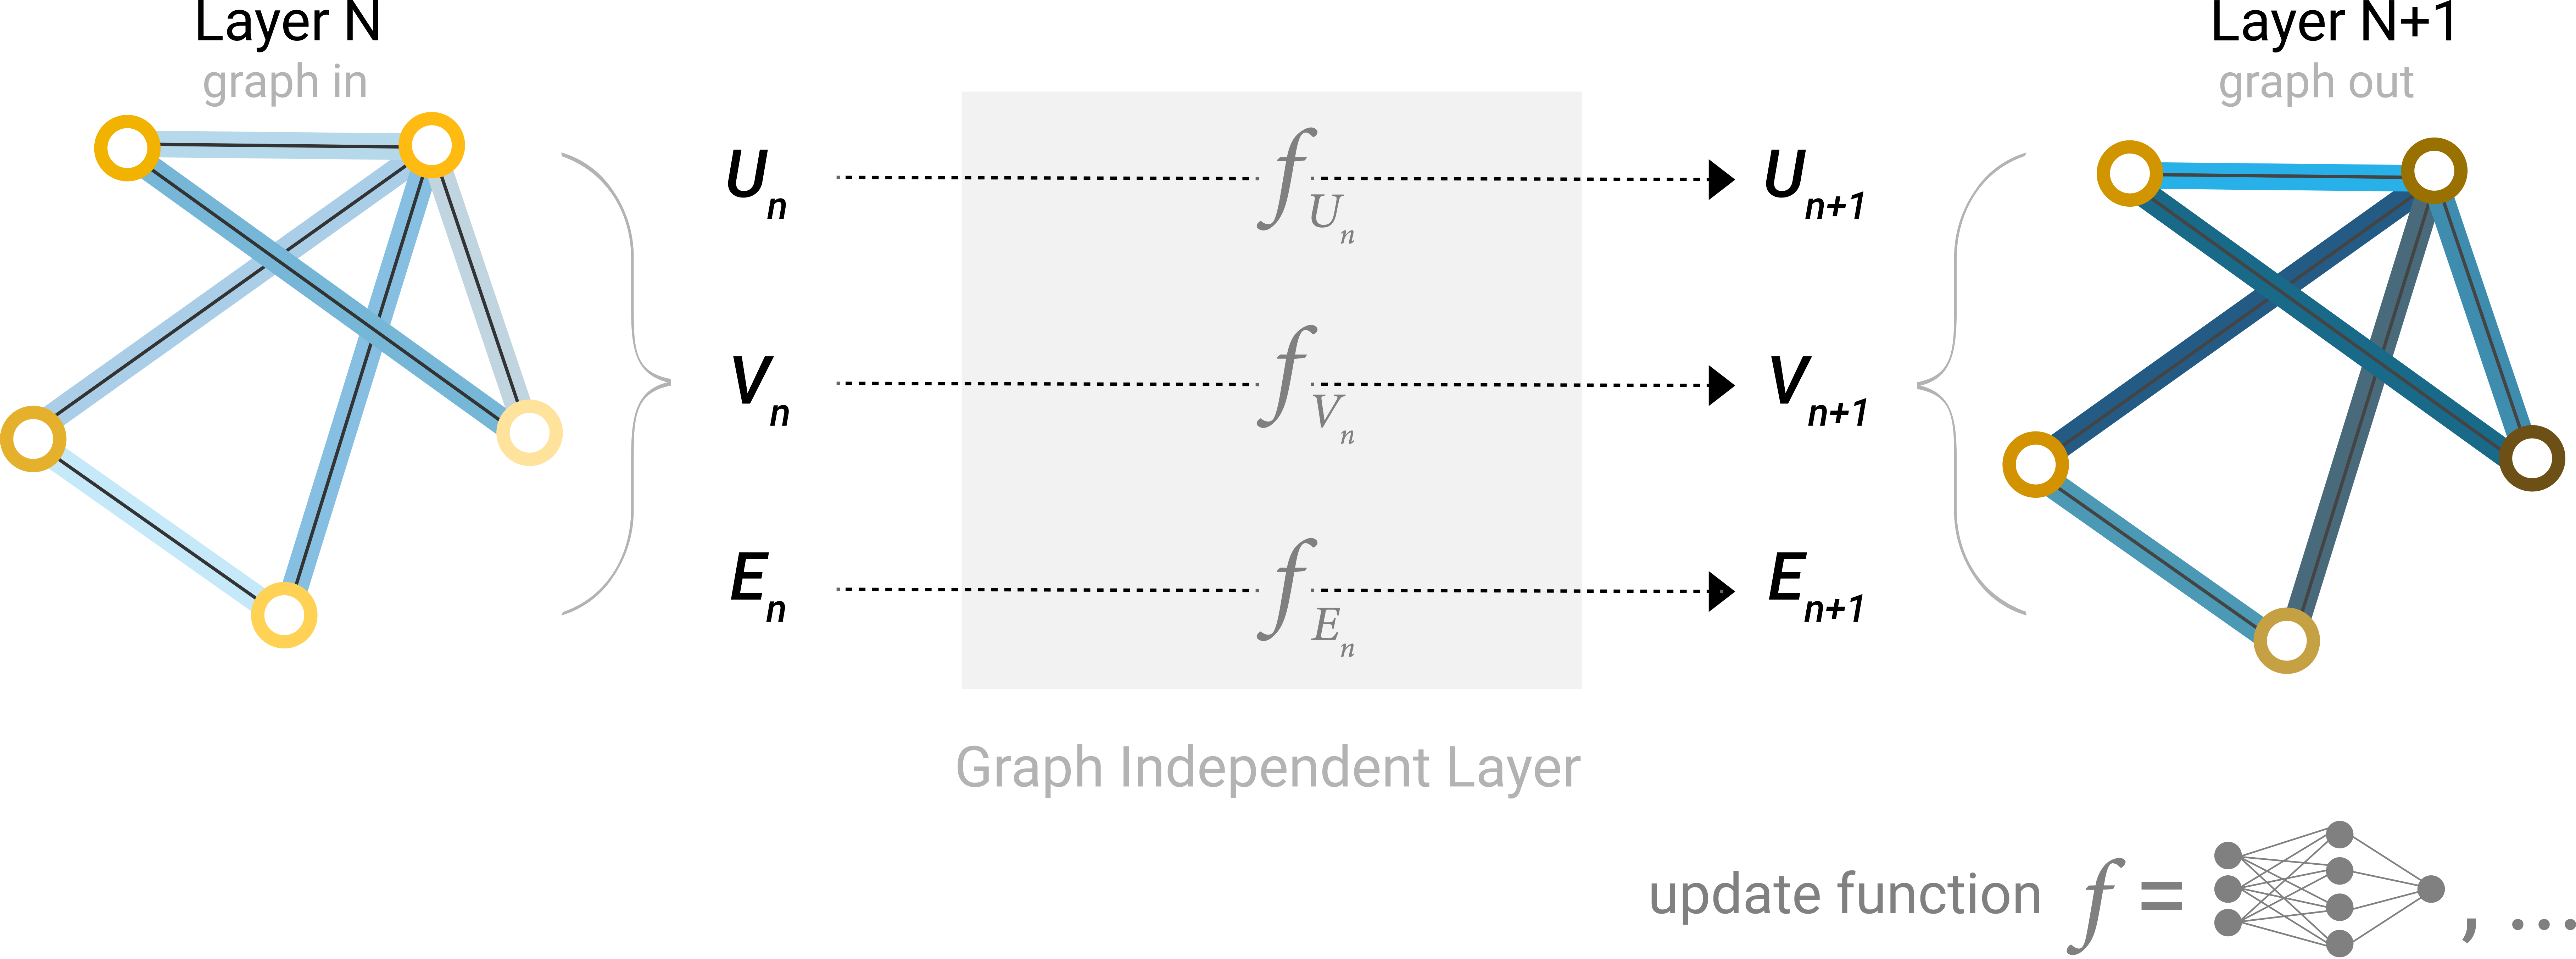
\includegraphics[width=\linewidth]{./assets/images/gnn-overall}
  \caption[Γενική δομή GNN]{Ένα GNN layer: Τα χαρακτηριστικά του γράφου διέρχονται από ένα MLP (βλ. Εν. \ref{ssec:nn}) και παράγουν έναν ανανεωμένο γράφο \cite{sanchez-lengeling2021a}.}
  \label{fig:gnn-overall}
\end{figure}

Η πρώτη αρχιτεκτονική GNNs εισήχθη το 2009 από τους Scarselli et al. \cite{scarselli_graph_2009} και η βασική αρχή της είναι ότι η κατάσταση κάθε κόμβου στο δίκτυο δεν καθορίζεται αυτόνομα, αλλά θα πρέπει να επηρεάζεται και από αυτή των γειτόνων του, καθώς είναι συνδεδεμένος με αυτούς τοπολογικά. Έτσι το δίκτυο «απορροφά» την τοπολογία του γράφου κατά την διαδικασία αλλαγής των βαρών του. Η τεχνική αυτή αναπτύχθηκε περαιτέρω, σχηματίζοντας τον μηχανισμό του Message Passing (\autoref{fig:message-passing}) \cite{gilmer_neural_2017}, δηλαδή της «ανταλλαγής μηνυμάτων» μεταξύ των κόμβων του δικτύου μέσω των ακμών που τους συνδέουν. Σε αυτό το πλαίσιο, κάθε κόμβος-στόχος $v$ ενημερώνει την κατάστασή του αντλώντας πληροφορία από τους συνδεδεμένους γείτονές του $u$. Ειδικότερα, για κάθε γείτονα παράγεται ένα «μήνυμα» μέσω μιας συνάρτησης $f_e(h_u, h_v, e_{uv})$, η οποία λαμβάνει υπόψη:
\begin{itemize}[noitemsep]
    \item την τρέχουσα κατάσταση του κόμβου-στόχου $h_v$,
    \item την τρέχουσα κατάσταση του γειτονικού κόμβου $h_u$,
    \item τα χαρακτηριστικά της μεταξύ τους ακμής $e_{uv}$.
\end{itemize}
Αυτά τα επιμέρους μηνύματα από όλους τους γείτονες συγκεντρώνονται μέσω μιας συνάρτησης συνάθροισης (aggregation function), όπως η μέση τιμή (mean) ή το μέγιστο (max). Τέλος, η αθροιστική πληροφορία περνά από μια συνάρτηση ανανέωσης (update function, συνήθως ένα μη γραμμικό νευρωνικό επίπεδο) και παράγεται η νέα κατάσταση του κόμβου $v$. Η επιλογή των συναρτήσεων εξαρτάται από την κάθε υλοποίηση. Ενδεικτικές αρχιτεκτονικές είναι τα Graph Convolutional Networks (GCNs) \cite{kipf_semi-supervised_2017}, τα Graph Attention Networks (GATs) \cite{velickovic_graph_2018} και το GraphSAGE \cite{hamilton_inductive_2017}.

Η διαδικασία αυτή εκτελείται ταυτόχρονα για όλους τους κόμβους του δικτύου. Με την ολοκλήρωση ενός επιπέδου του GNN, κάθε κόμβος έχει ενσωματώσει πληροφορία από τους άμεσους ($1$-hop) γείτονές του. Η προσθήκη πολλαπλών επιπέδων επιτρέπει στο δίκτυο να αντλήσει πληροφορία από έμμεσους γείτονες (τους γείτονες των γειτόνων κάθε κόμβου). Γενικεύοντας, ένα GNN $k$ επιπέδων καθορίζει την επόμενη κατάσταση κάθε κόμβου από αυτή των $k$-hop γειτόνων του. Παρότι περισσότερα επίπεδα επιτρέπουν την κατανόηση βαθύτερων δομών, αυξάνουν δραματικά το υπολογιστικό κόστος και συχνά οδηγούν στο φαινόμενο του oversmoothing \cite{li_deeper_2018} των χαρακτηριστικών κάθε κόμβου, γι' αυτό και πρακτικά τα περισσότερα GNNs περιορίζονται σε 2 ή 3 επίπεδα.

\begin{figure}[htbp]
  \centering
  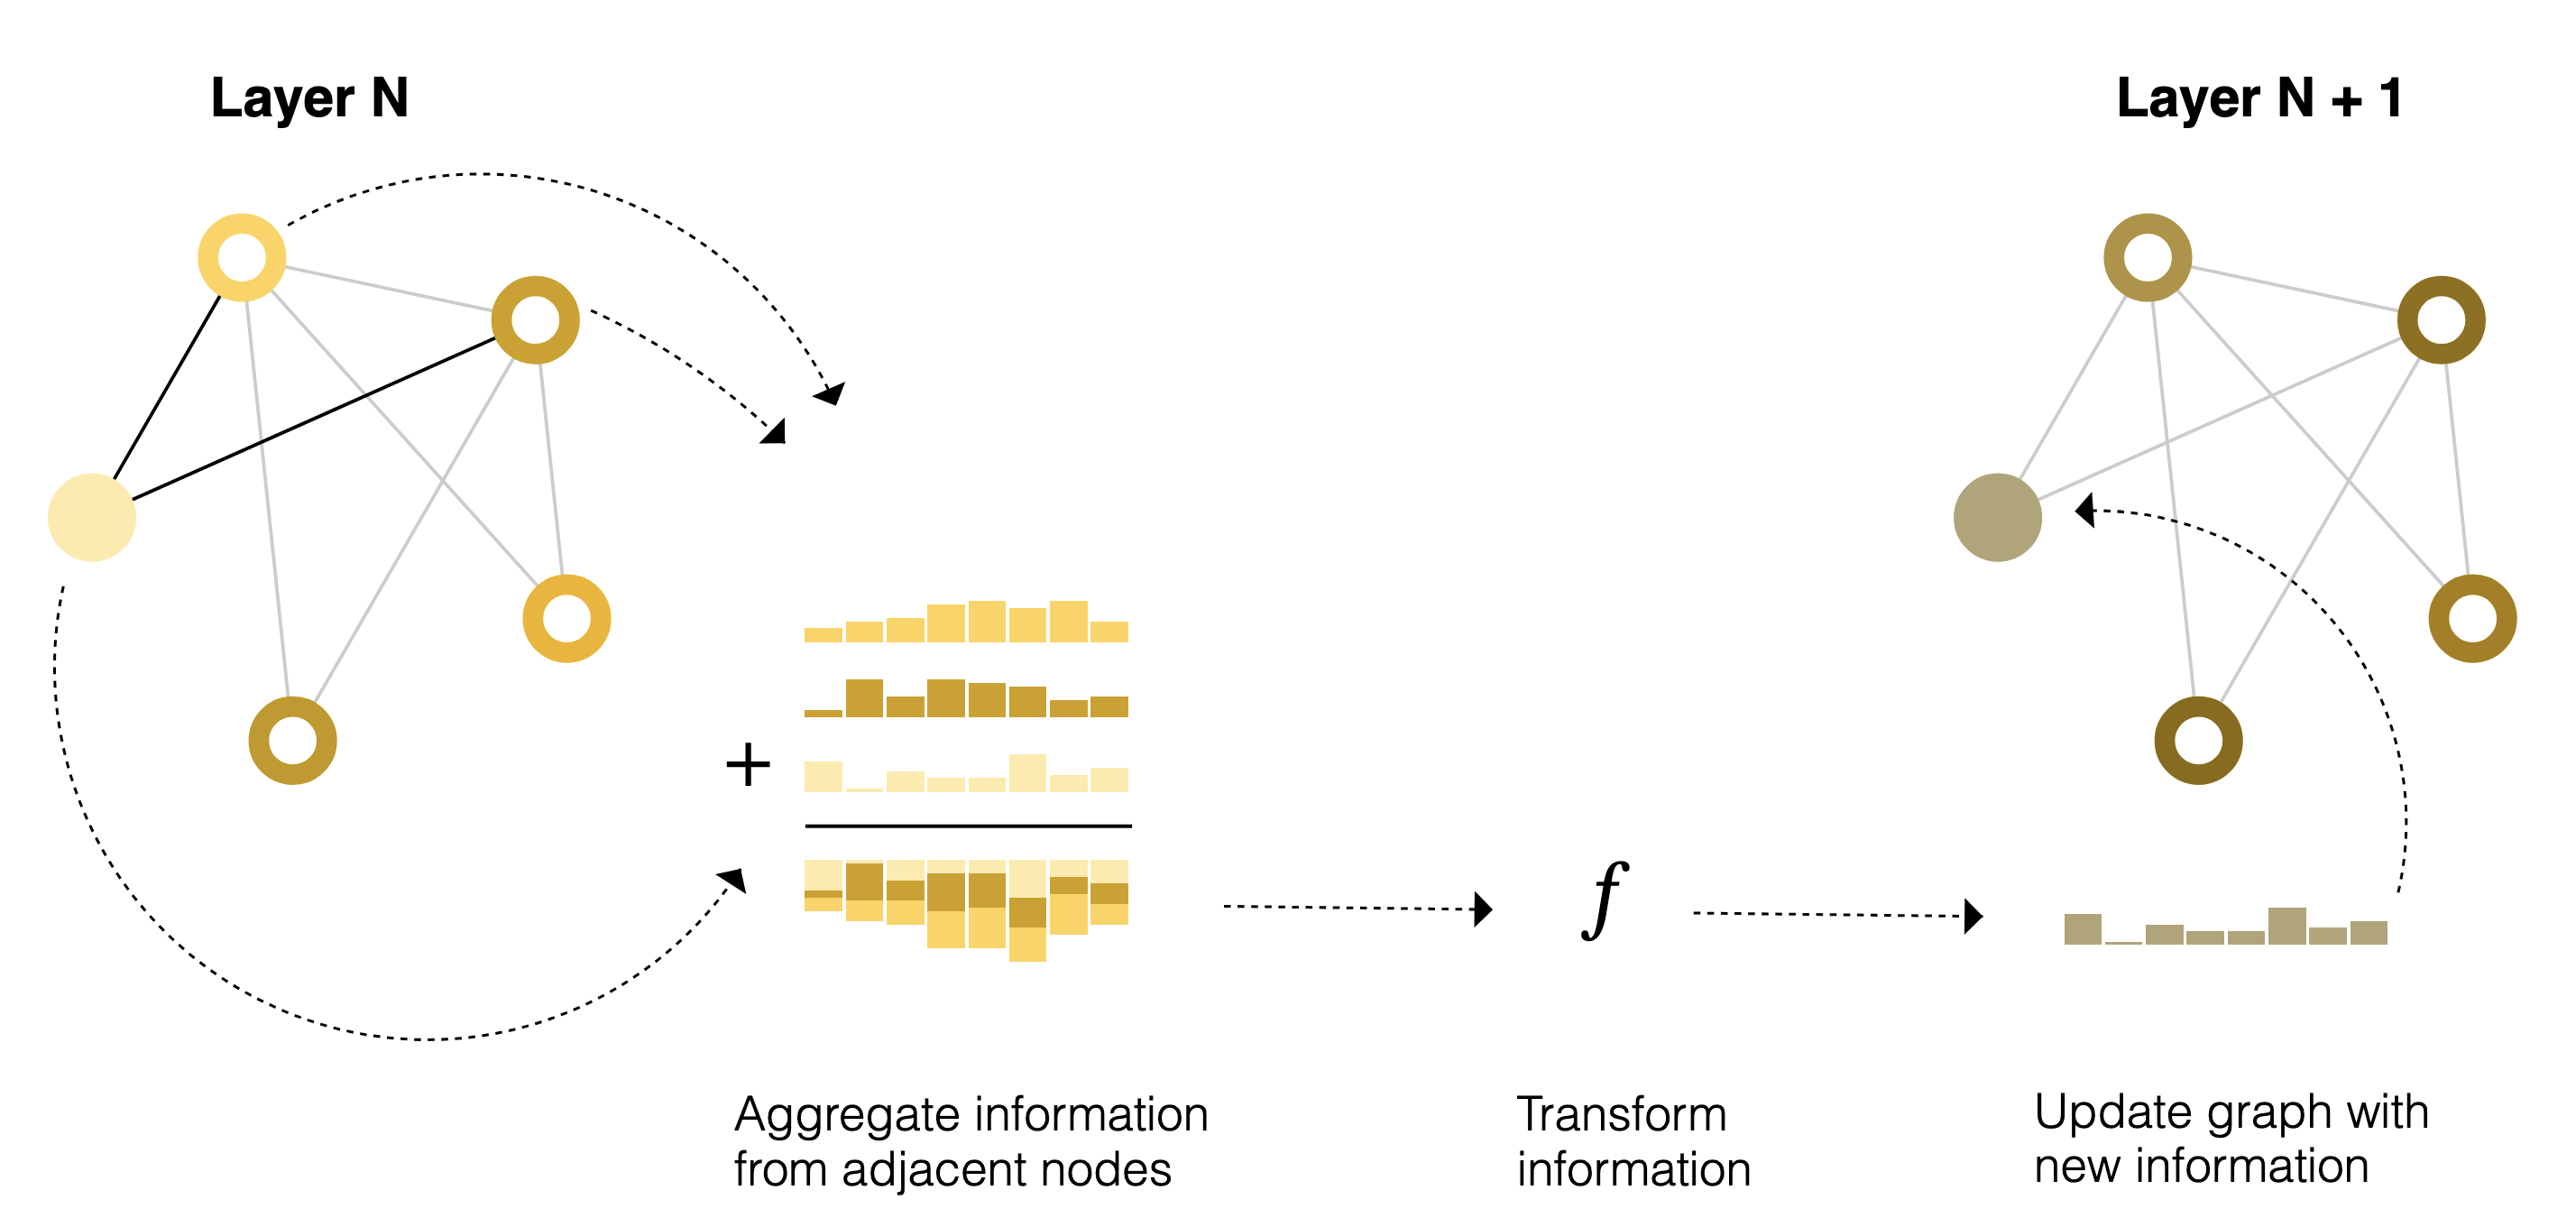
\includegraphics[width=\linewidth]{./assets/images/message-passing}
  \caption[Message passing στα GNNs]{Η διαδικασία του message passing: ο κόμβος με γέμισμα (αριστερά) κάνει aggregate πληροφορία από τον εαυτό του και τους δύο γείτονές του και ανανεώνει την κατάστασή του (δεξιά) μέσω μίας update function. Η διαδικασία γίνεται σε κάθε κόμβο του γράφου \cite{sanchez-lengeling2021a}.}
  \label{fig:message-passing}
\end{figure}

Μία αρχιτεκτονική που αξίζει περαιτέρω ανάπτυξη, καθώς χρησιμοποιείται στην μεθοδολογία της παρούσας διπλωματικής, είναι αυτή του GraphSAGE (Sample and Aggregate) (\autoref{fig:graphsage}) \cite{hamilton_inductive_2017}. Ο αλγόριθμος σχεδιάστηκε για να παράγει embeddings επαγωγικά μέσα από την επαναληπτική διαδικασία τριών βημάτων που αναφέρθηκε παραπάνω: sampling, aggregation, update:
\begin{enumerate}
    \item \textbf{Sampling:} Το δίκτυο δεν εξετάζει το σύνολο των κόμβων που συνδέονται με τον $v$, αλλά επιλέγει τυχαία ένα σταθερό πλήθος γειτόνων $u$.
    \item \textbf{Aggregation:} Στη συνέχεια, τα χαρακτηριστικά αυτών των γειτόνων $u$ συγκεντρώνονται σε ένα ενιαίο διάνυσμα μέσω μιας aggregation function, συνήθως της μέσης τιμής (mean aggregation).
    \item \textbf{Update:} Αφού εξαχθεί η πληροφορία των γειτόνων, παράγεται η συνένωση (concatenation) του τρέχοντος διανύσματος του κόμβου $v$ με το νέο, συναθροισμένο διάνυσμα των γειτόνων του και το αποτέλεσμα πολλαπλασιάζεται με τον πίνακα βαρών του συγκεκριμένου επιπέδου και διέρχεται από μία μη γραμμική συνάρτηση ενεργοποίησης (συνήθως ReLU), παράγοντας την τελική ανανεωμένη αναπαράσταση του κόμβου.
\end{enumerate}
Επαναλαμβάνοντας αυτή τη διαδικασία για $k$ επίπεδα (όπου συνήθως $k=2$), ο τελικός κόμβος αποκτά ένα embedding που έχει ενσωματώσει επιτυχώς τόσο τα δικά του χαρακτηριστικά, όσο και την συντακτική και τοπολογική δομή της άμεσης και έμμεσης γειτονιάς του.

\begin{figure}[htbp]
  \centering
  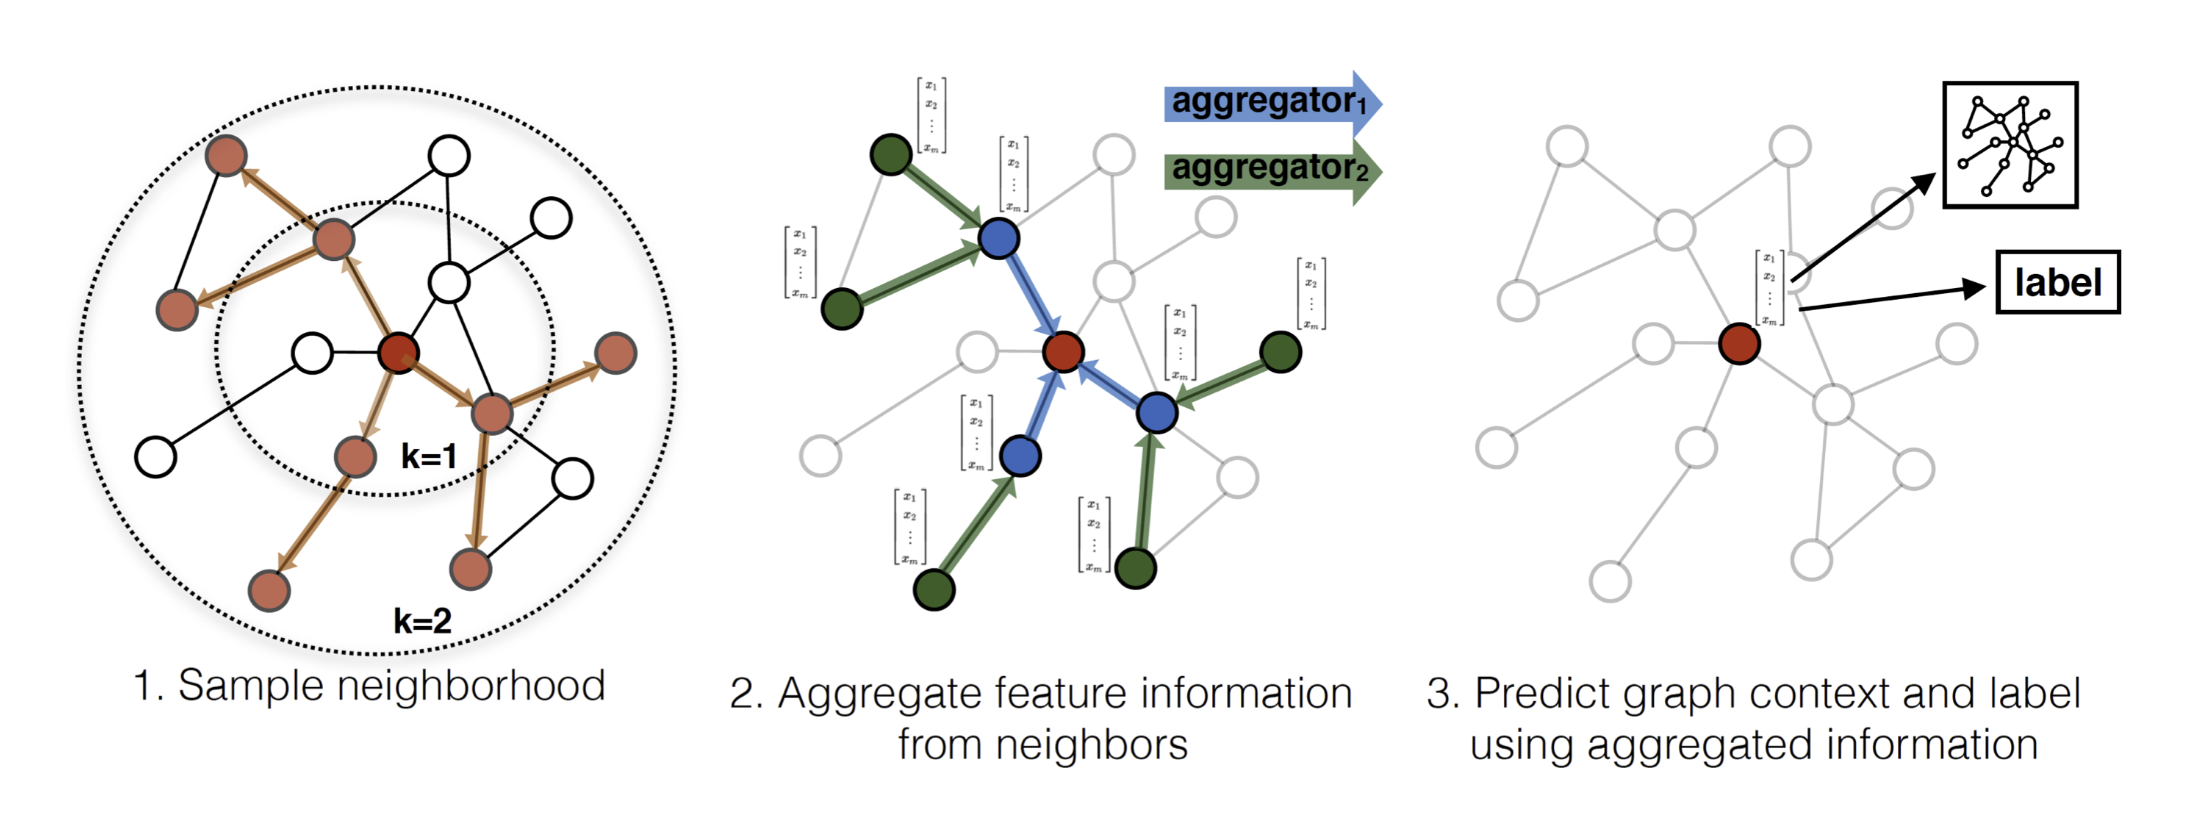
\includegraphics[width=\linewidth]{./assets/images/graphsage}
  \caption[Το pipeline του GraphSAGE]{Τα τρία βήματα του GraphSAGE: sampling γειτόνων, aggregation και update \cite{hamilton_inductive_2017}.}
  \label{fig:graphsage}
\end{figure}

Ανεξαρτήτως της επιμέρους αρχιτεκτονικής, τα embeddings που παράγει ένα GNN αποτελούν τη βάση για το τελικό ζητούμενο, την πρόβλεψη: ένα τελικό επίπεδο (π.χ. ένα MLP) τα αξιοποιεί ώστε να παραγάγει προβλέψεις σε επίπεδο κόμβου, ακμής ή ολόκληρου του γράφου (\autoref{fig:gnn-prediction}). Στην παρούσα εργασία το ζητούμενο είναι η πρόβλεψη νέων ακμών, δηλαδή νέων κανόνων μεταξύ των συσκευών ενός χρήστη.

\begin{figure}[htbp]
  \centering
  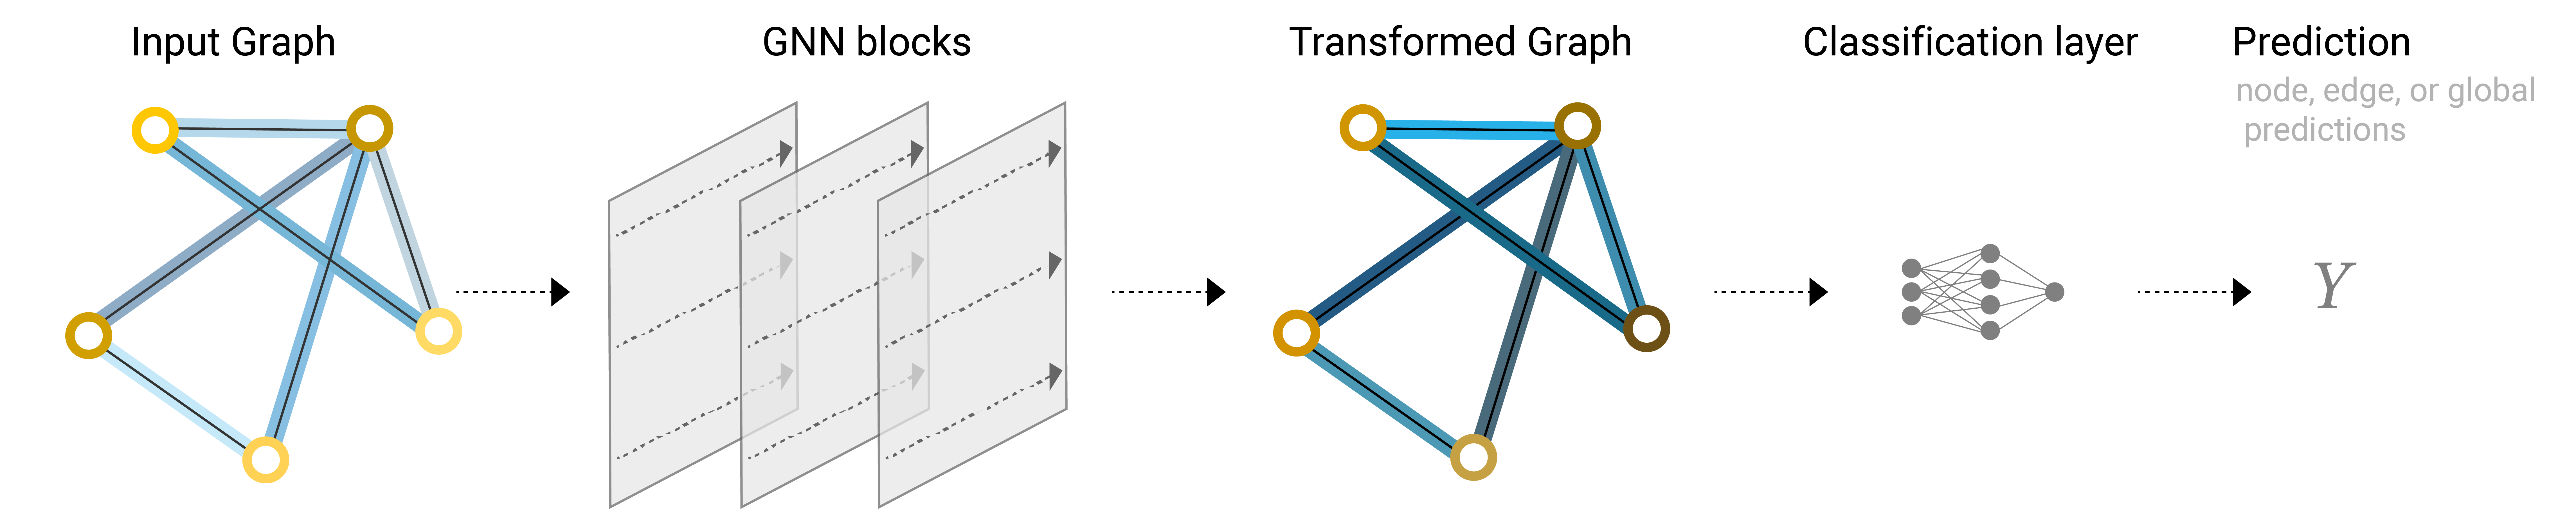
\includegraphics[width=\linewidth]{./assets/images/gnn-prediction}
  \caption[Χρήση GNN για πρόβλεψη]{Αξιοποίηση ενός GNN για πρόβλεψη: τα embeddings που παράγονται από τα επίπεδα message passing τροφοδοτούν ένα τελικό επίπεδο πρόβλεψης \cite{sanchez-lengeling2021a}.}
  \label{fig:gnn-prediction}
\end{figure}

\section{Συστήματα Σύστασης}\label{sec:recsys}
Στις ακόλουθες παραγράφους επεξηγείται το πρόβλημα της παραγωγής προτάσεων και η δομή των Συστημάτων Σύστασης (Recommender Systems) \cite{ricci_recommender_2011}, καθώς και η άμεση εφαρμογή τους στα IoT οικοσυστήματα. Τα Συστήματα Σύστασης είναι ένα πεδίο της επιστήμης της Ανάλυσης Δεδομένων το οποίο ασχολείται με τον εντοπισμό λανθανόντων μοτίβων από μεγάλα σύνολα δεδομένων χρηστών, με σκοπό το προσωποποιημένο φιλτράρισμα πληροφορίας. Η κεντρική ιδέα είναι η μελέτη και αξιολόγηση των επιλογών κάθε χρήστη με βάση το δικό του ιστορικό και τα γενικευμένα μοτίβα του συνόλου. Για παράδειγμα, μία μηχανή αναζήτησης ταινιών εξετάζει το ιστορικό και τις βαθμολογίες που έχει δώσει ήδη ο εκάστοτε χρήστης (content-based filtering), υπολογίζει τον βαθμό ομοιότητάς του με άλλους χρήστες (collaborative filtering), και του προτείνει μια νέα ταινία με στατιστικά πολύ μεγαλύτερη πιθανότητα να τον ικανοποιήσει απ' ό,τι μια τυχαία επιλογή.

\begin{figure}[htbp]
  \centering
  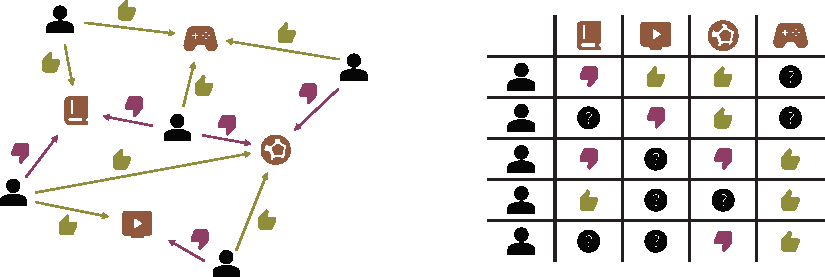
\includegraphics[width=0.95\linewidth]{./assets/images/recsys}
  \caption[Συστήματα σύστασης]{Επισκόπηση ενός συστήματος σύστασης: Αρχικά, οι χρήστες δηλώνουν τις προτιμήσεις τους (αριστερά). Στην συνέχεια το σύστημα προβλέπει τις προτιμήσεις κάθε χρήστη για τα αντικείμενα που δεν έχει βαθμολογήσει ακόμη (ερωτηματικά στον πίνακα δεξιά).}
  \label{fig:recsys}
\end{figure}

Στα IoT οικοσυστήματα, που αποτελούν και το αντικείμενο της παρούσας εργασίας, τα συστήματα σύστασης έρχονται να επιλύσουν το πρόβλημα της αδράνειας χρηστών. Αυτό που κάνει τις IoT συσκευές «έξυπνες» είναι η δυνατότητά τους να αυτοματοποιούνται. Για παράδειγμα, ένας έξυπνος θερμοστάτης διαφοροποιείται από έναν συμβατικό διότι μπορεί να ενεργοποιείται ασύρματα βάσει γεωγραφικής θέσης ή συγκεκριμένου χρονοδιαγράμματος και να λειτουργεί συνεργατικά με άλλες έξυπνες συσκευές όπως λαμπτήρες ή αισθητήρες κίνησης, με βάση ορισμένους κανόνες. Η διαχείριση τέτοιων κανόνων ωστόσο εναπόκειται συνήθως στους ίδιους τους χρήστες, οι περισσότεροι εκ των οποίων καταλήγουν να ορίζουν ελάχιστους ή και κανέναν, με αποτέλεσμα οι συσκευές να υπολειτουργούν ως απλά, τηλεχειριζόμενα εργαλεία. Εδώ ακριβώς έγκειται η αξία της έξυπνης σύστασης κανόνων (rule recommendation): η αυτοματοποίηση του ίδιου του συστήματος αυτοματοποίησης.

Οι αρχιτεκτονικές που χρησιμοποιούνται για την παραγωγή προτάσεων ποικίλλουν δραστικά \cite{adomavicius_toward_2005}, από αμιγώς στατιστικές μεθόδους παραγοντοποίησης πινάκων (matrix factorization) (περαιτέρω ανάλυση στην \autoref{sec:problem-model}) έως βαθιά Νευρωνικά Δίκτυα. Ο στόχος τους όμως είναι πάντοτε ο ίδιος: δεδομένης της υπάρχουσας τοπικής πληροφορίας (ποιες συσκευές και ποιους κανόνες κατέχει ήδη ο χρήστης), και λαμβάνοντας υπόψη την πληροφορία όλων των χρηστών (ποιοι κανόνες εμφανίζονται συχνότερα στο σύνολο του δικτύου), το σύστημα προβλέπει και προτείνει στον χρήστη τον νέο κανόνα που έχει την μεγαλύτερη πιθανότητα να είναι του χρήσιμος.

Ολοκληρώνοντας το παρόν Κεφάλαιο, έχουν τεθεί πλέον όλα τα θεωρητικά θεμέλια για τη μοντελοποίηση του προβλήματος που καλείται να επιλύσει η παρούσα εργασία: η ανάπτυξη ενός συστήματος σύστασης για IoT οικοσυστήματα, το οποίο μοντελοποιεί ένα δοθέν σύνολο δεδομένων ως γράφους και εκπαιδεύει ένα μοντέλο GNN μέσα σε ένα ομοσπονδιακό περιβάλλον, με στόχο την διασφάλιση όχι μόνο της υψηλής υπολογιστικής αποδοτικότητας αλλά και της προστασίας της ιδιωτικότητας των χρηστών.
